\documentclass[11pt]{article}

 	\usepackage{natbib}
    \usepackage[usenames, dvipsnames]{color}
    %\bibliographystyle{apj}
    
    \usepackage[T1]{fontenc}
    % Nicer default font (+ math font) than Computer Modern for most use cases
    \usepackage{mathpazo}

    % Basic figure setup, for now with no caption control since it's done
    % automatically by Pandoc (which extracts ![](path) syntax from Markdown).
    \usepackage{graphicx}

    \usepackage{geometry} % Used to adjust the document margins
    \usepackage{amsmath} % Equations
    \usepackage{amssymb} % Equations
    
    \usepackage[mathletters]{ucs} % Extended unicode (utf-8) support
    \usepackage[utf8x]{inputenc} % Allow utf-8 characters in the tex document
    \usepackage{fancyvrb} % verbatim replacement that allows latex
    \usepackage{grffile} % extends the file name processing of package graphics 
                         % to support a larger range 
    % The hyperref package gives us a pdf with properly built
    % internal navigation ('pdf bookmarks' for the table of contents,
    % internal cross-reference links, web links for URLs, etc.)
    \usepackage{hyperref}
    \usepackage[normalem]{ulem} % ulem is needed to support strikethroughs (\sout)
                                % normalem makes italics be italics, not underlines
    \usepackage{caption}
	\usepackage{subcaption}
    \usepackage{fancyhdr} 
    \usepackage{wrapfig,booktabs}

	\newcommand{\numpy}{{\tt numpy}}    % tt font for numpy

\topmargin -.5in
\textheight 9in
\oddsidemargin -.25in
\evensidemargin -.25in
\textwidth 7in

\begin{document}

% ========== Edit your name here
\author{Natalie Price-Jones}
\title{Review: Summer 2019}
\maketitle

\medskip

I have engaged in two main areas of research this summer. My primary effort was put towards manipulating chemical abundances from APOGEE \citep{Majewski2015} so that I could apply DBSCAN \citep{Ester1996} to those abundances and identify over-densities in chemical space. This meant making a significant number of quality cuts on the data. At a minimum, I wanted to find stars with a measurement for each abundance of interest. Depending on the number of abundances I wanted to use for clustering, this might mean cutting a great many stars (more than 80\% for 15 abundances) from the sample. I also wanted to ensure that the abundances I used were well measured, and so incorporated minimum cuts on signal to noise ratio of the observed spectra from which the abundances were derived, as well as cutting out stars with poorly measured surface gravities or effective temperatures. As those photospheric properties have a global effect on the spectrum, it was crucial to also limit myself to stars within ranges where I expected good results from the APOGEE pipeline. 

\begin{figure}
  \centering
  \begin{subfigure}[b]{0.45\textwidth}
    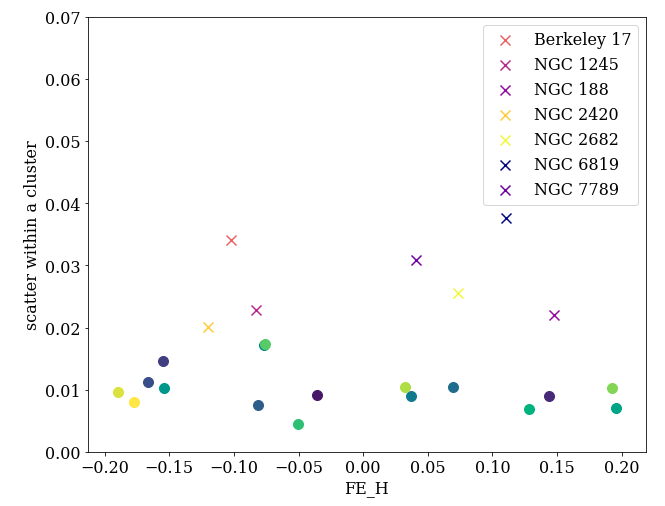
\includegraphics[width=\textwidth]{compactness.png}
   \caption{iron abundance.}
  \label{fig:fecompact}
  \end{subfigure}
\hfill
  \begin{subfigure}[b]{0.45\textwidth}
    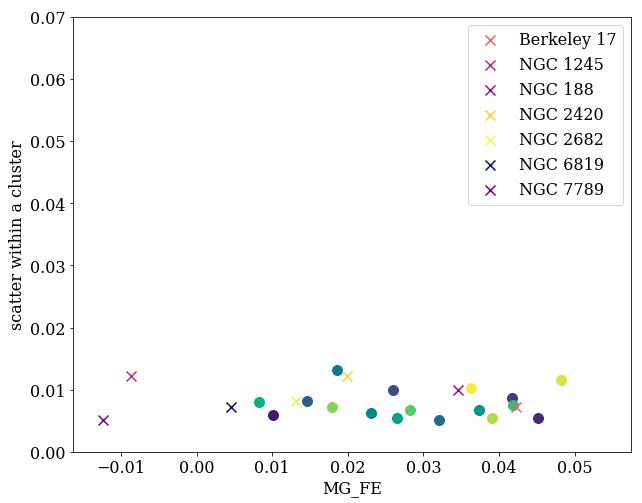
\includegraphics[width=\textwidth]{mgcompactness.png}
  \caption{magnesium abundance.}  
  \label{fig:mgcompact}
  \end{subfigure}
  \hfill
    \caption{Standard deviation in abundance among stars in a group as a function of mean abundance for that group. Circles are groups found by DBSCAN, coloured by their label number, while crosses are open clusters, identified from the OCCAM catalogue \citep{Donor2018}}
    \label{fig:compact}
\end{figure}


Once I had completed these quality cuts, I ran several instances of DBSCAN, using what I had learned from my simulations in \citep{Price-Jones2019} to choose the appropriate values for DBSCAN parameters $\epsilon$ (the radius around each star to consider) and $N_{\rm pts}$ (the number of points within $\epsilon$ that identified a cluster star). In simulations, the recovery fraction (fraction of input clusters successfully found by DBSCAN) was maximized when I chose an $\epsilon$ and $N_{\rm pts}$ that maximized the total number of clusters found. I made the same choice for DBSCAN parameters when working with the real data. Also as in my simulations, $\epsilon\equiv n\cdot d_{\rm typ}$ where $d_{\rm typ}$ is the median pairwise distance between points and $n$ was the `neighbourhood scale', the quantity I varied when trying to find the best parameterization of DBSCAN. When working with the real data, the best scale was typically $n\sim0.015$.

Once groups were found by DBSCAN, I limited my analysis to those groups with more than 15 members. I then cut to groups with a silhouette coefficient greater than zero. The silhouette coefficient is the ratio of the typical distance between members of a group to the typical distance between members of that group and members of other nearby groups. The higher the silhouette coefficient, the more distinct a group is, and the less overlap it has with non-member stars. Cutting on this value allowed me to remove a common result of DBSCAN; one overly large group that spanned most of the chemical space. It was surprising that such a group was produced given the prevalence of smaller ones, and I plan to investigate how such a group crumbles under changing $n$.

Initially my interest was in comparing my groups to open clusters, as I had hoped to recover some of them in my analysis. I did not successfully find any groups that could be matched with more than one member to an open cluster. In addition, the groups I found were more tightly clustered in some abundance spaces than the open clusters. Figure~\ref{fig:fecompact} shows this effect for iron. However in other elements, like magnesium, the compactness was much more comparable (Figure~\ref{fig:mgcompact}). This effect is significant enough that it is visible when just looking at the projection of this space and colour-coding points by their membership, as I did for Figure~\ref{fig:alphafe}.

\begin{figure}
  \begin{center}
    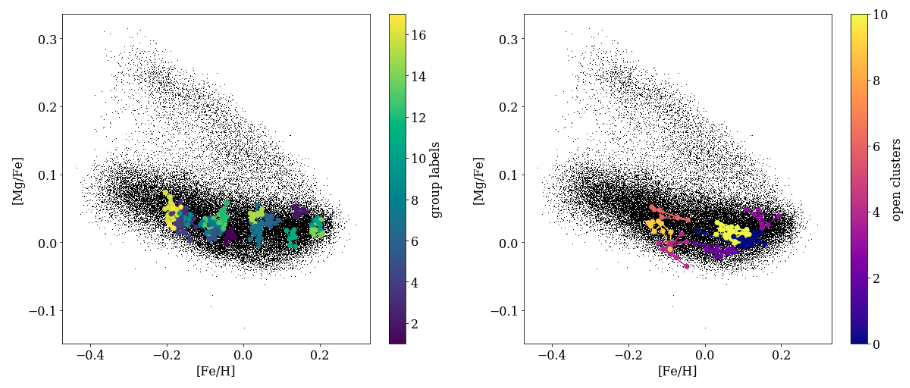
\includegraphics[width=\textwidth]{mgvsfe.png}
  \end{center}
  \caption{[Mg/Fe] vs [Fe/H] for stars in the APOGEE survey that met my quality cuts (black points). Coloured points are stars that are associated with each other. On the left, these are groups found by DBSCAN, while on the right are open clusters. As we see in Figure~\ref{fig:fecompact}, the groups are typically less spread out in [Fe/H] than the open clusters. }
  \label{fig:alphafe}
\end{figure}

This result is not necessarily unexpected, but given the well established homogeneity of open clusters in chemical space, I was prompted to dig deeper. In particular, I was hoping to investigate with more stars, and began updating my code to work with APOGEE's newest internal data release, DR16. I also moved from using the abundances produced by APOGEE's pipeline, ASPCAP \citep{aspcap} to using those from \texttt{astroNN} \citep{astronn}. While I was able to gain some stars this way, it seemed the primary thing holding me back was using many elements and keeping tight restrictions on measurement uncertainties. By reducing the number of elements used and increasing the maximum allowed uncertainty I could increase the number of stars I was using from my sample (although not as much as expected, even with relaxed quality cuts). I was still unable to recover any open clusters, and began to experiment with testing DBSCAN on other distributions. As a sanity check, I used Gaussian mixture modelling (GMM) to model the observed abundances as a combination of three multivariate Gaussians. I then sampled points from this combinations of Gaussians until I had the same number of stars as I did in the real APOGEE data. Applying DBSCAN to this data randomly sampled from a smooth distribution still gave me groups. Not only that but the number of groups identified was within 10 of number found in the real data. This seems inherently problematic; if DBSCAN can find groups in random data, perhaps the groups it finds in the APOGEE data are just as artificial.

To better understand this, I plan to increase the number of points sampled in the GMM-data to see if it reaches some point where the smoothness is sufficiently well characterized that DBSCAN cannot find groups. I also plan to investigate the groups that I do find in the real data, to try and understand their kinematic properties through measurements from Gaia. 

In addition to this work on applying DBSCAN to APOGEE data, I spent part of the summer working with Itamar Reis on using his probabilistic random forest (PRF-\citealt{Reis2018}) code to provide an alternative way to measure the distance between stars. At present, I compute Euclidean distances between the stars in the abundance spaces I use. However, as I proceed to higher dimensional spaces, this becomes problematic; distances no longer behave as expected from our three dimensional intuition. Using an alternative distance metric offered another way to understand the high dimensional chemical space I explore with chemical tagging.

This work is still on-going; PRF has tuneable hyper-parameters which must be set, and early results have done worse than Euclidean distances in finding a significant number of groups in simulated data. However, developing alternate distance metrics is crucial, as DBSCAN does not incorporate uncertainties into its cluster assignments. Changing the distance metric used might offer a way to make use of the measured uncertainties on the chemical space positions of stars. For highly uncertain measurements, this approach may still allow probabilistic cluster assignment, rather than the binary membership status I currently produce.

I am optimistic that during the fall semester I will be able to sufficiently characterize my DBSCAN-identified groups in the APOGEE data and draft a paper describing not only what I have found in my efforts with DBSCAN, but what can be expected from future spectroscopic surveys like MWM \citep{Kollmeier2017}. In addition, I would like to advance my simulated data to more explicitly include the impact of radial migration as it is often prescribed in the literature, and perhaps include simulated photometry for my stars. Working with Jeremy on solar siblings has also got me interested in trying to understand the evolution of an individual cluster and I would like to continue to meet regularly with him to understand how I might be able to incorporate more kinematics into my simulations without having to go full N-body. 

\bibliographystyle{apj}
\bibliography{sim}

\end{document}
\grid
\grid